%==============================================================================
% Chapitre 44 - Le projectile dans la cartouche
%==============================================================================

\section{Introduction}

Le projectile constitue l'élément destiné à quitter l'arme et à atteindre la
cible.

Cependant, avant son départ, il fait partie intégrante de la cartouche.

Sa position, son maintien et son assemblage influencent directement les
performances balistiques.

\begin{aretenir}

Le comportement d'un projectile dépend non seulement de sa géométrie mais
également de la manière dont il est assemblé dans la cartouche.

\end{aretenir}

\section{Le projectile dans la chaîne balistique}

Nous avons déjà étudié en détail :

\begin{itemize}
    \item la géométrie ;
    \item la masse ;
    \item la stabilité ;
    \item les propriétés aérodynamiques.
\end{itemize}

Dans ce chapitre, nous nous intéressons à son intégration dans la munition.

\section{Position dans l'étui}

Le projectile est maintenu dans le collet de l'étui.

Une partie du projectile demeure à l'intérieur de l'étui tandis qu'une autre
reste visible à l'extérieur.

Cette position influence directement :

\begin{itemize}
    \item la longueur totale de la cartouche ;
    \item le volume disponible pour la poudre ;
    \item l'alimentation de l'arme.
\end{itemize}

\section{Longueur totale}

La longueur totale de cartouche est souvent désignée par l'acronyme anglais :

\begin{quote}
OAL (\emph{Overall Length})
\end{quote}

ou :

\begin{quote}
COL (\emph{Cartridge Overall Length})
\end{quote}

Cette dimension joue un rôle essentiel dans le fonctionnement des armes.

\section{Importance de la longueur totale}

Une longueur incorrecte peut provoquer :

\begin{itemize}
    \item des incidents d'alimentation ;
    \item des problèmes de chambrage ;
    \item des variations de pression ;
    \item une dégradation de la précision.
\end{itemize}

Les fabricants définissent donc des limites précises.

\section{Enfoncement du projectile}

L'enfoncement correspond à la profondeur d'insertion du projectile dans
l'étui.

Cette grandeur influence directement :

\begin{itemize}
    \item le volume interne disponible ;
    \item la pression maximale ;
    \item la combustion de la poudre.
\end{itemize}

\begin{figure}[htbp]
\centering

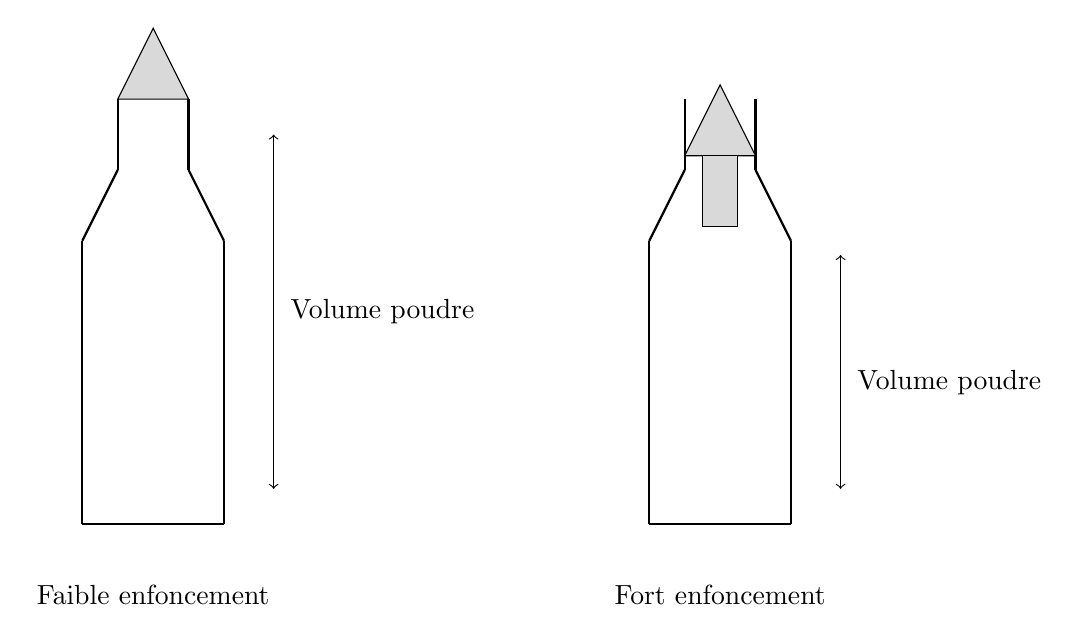
\begin{tikzpicture}[scale=0.9]

% Cartouche gauche
\draw[thick] (0,0) -- (0,4);
\draw[thick] (2,0) -- (2,4);
\draw[thick] (0,0) -- (2,0);

\draw[thick] (0,4) -- (0.5,5);
\draw[thick] (2,4) -- (1.5,5);

\draw[thick] (0.5,5) -- (0.5,6);
\draw[thick] (1.5,5) -- (1.5,6);

% Projectile peu enfoncé
\draw[fill=gray!30] (0.5,6) -- (1,7) -- (1.5,6) -- cycle;

\node at (1,-1) {Faible enfoncement};

% Flèche volume
\draw[<->] (2.7,0.5) -- (2.7,5.5);
\node[right] at (2.8,3) {Volume poudre};

% Cartouche droite
\begin{scope}[xshift=8cm]

\draw[thick] (0,0) -- (0,4);
\draw[thick] (2,0) -- (2,4);
\draw[thick] (0,0) -- (2,0);

\draw[thick] (0,4) -- (0.5,5);
\draw[thick] (2,4) -- (1.5,5);

\draw[thick] (0.5,5) -- (0.5,6);
\draw[thick] (1.5,5) -- (1.5,6);

% Projectile fortement enfoncé
\draw[fill=gray!30]
(0.5,5.2) --
(1,6.2) --
(1.5,5.2) --
cycle;

\draw[fill=gray!30]
(0.75,4.2)
rectangle
(1.25,5.2);

\node at (1,-1) {Fort enfoncement};

\draw[<->] (2.7,0.5) -- (2.7,3.8);
\node[right] at (2.8,2) {Volume poudre};

\end{scope}

\end{tikzpicture}

\caption{Influence de l'enfoncement du projectile sur le volume disponible pour la poudre.}
\label{fig:enfoncement_volume}
\end{figure}

\section{Volume disponible}

Lorsque l'enfoncement augmente :

\begin{itemize}
    \item le volume interne diminue ;
    \item la densité de chargement augmente ;
    \item la pression peut augmenter.
\end{itemize}

Cette relation est particulièrement importante en rechargement.

\begin{attention}

Une modification importante de l'enfoncement peut entraîner des variations
significatives de pression.

\end{attention}

\section{Maintien du projectile}

Le projectile doit être maintenu fermement dans le collet.

Ce maintien doit être suffisant pour :

\begin{itemize}
    \item résister aux manipulations ;
    \item supporter le recul ;
    \item garantir une mise à feu régulière.
\end{itemize}

\section{Tension de collet}

La tension de collet correspond à l'effort exercé par le collet sur le
projectile.

Elle dépend notamment :

\begin{itemize}
    \item du diamètre du projectile ;
    \item des dimensions du collet ;
    \item des propriétés mécaniques de l'étui.
\end{itemize}

\section{Influence sur la précision}

Une tension de collet régulière contribue à :

\begin{itemize}
    \item une combustion plus homogène ;
    \item une meilleure régularité des vitesses ;
    \item une meilleure précision.
\end{itemize}

\section{Alignement}

Le projectile doit être correctement aligné avec l'axe de l'étui.

Un mauvais alignement peut entraîner :

\begin{itemize}
    \item une entrée asymétrique dans les rayures ;
    \item une augmentation de la dispersion ;
    \item une perte de précision.
\end{itemize}

\section{Distance aux rayures}

Une fois chambrée, la cartouche positionne le projectile à une certaine
distance des rayures.

Cette distance est parfois appelée :

\begin{quote}
\emph{jump}
\end{quote}

dans la littérature anglo-saxonne.

\section{Influence du jump}

Le jump influence notamment :

\begin{itemize}
    \item la pression ;
    \item la précision ;
    \item le comportement du projectile au départ du coup.
\end{itemize}

Son optimisation constitue un sujet important en rechargement de précision.

\begin{figure}[htbp]
\centering

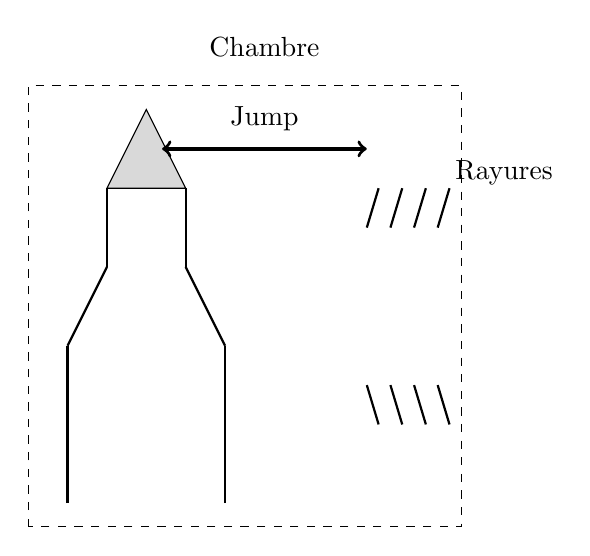
\begin{tikzpicture}[scale=1]

% Cartouche
\draw[thick] (0,0) -- (0,2);
\draw[thick] (2,0) -- (2,2);

\draw[thick] (0,2) -- (0.5,3);
\draw[thick] (2,2) -- (1.5,3);

\draw[thick] (0.5,3) -- (0.5,4);
\draw[thick] (1.5,3) -- (1.5,4);

% Projectile
\draw[fill=gray!30]
(0.5,4) --
(1,5) --
(1.5,4) --
cycle;

% Chambre
\draw[dashed] (-0.5,-0.3) rectangle (5,5.3);

\node at (2.5,5.8) {Chambre};

% Rayures
\foreach \x in {3.8,4.1,4.4,4.7}
{
    \draw[thick]
    (\x,3.5) --
    (\x+0.15,4.0);

    \draw[thick]
    (\x,1.5) --
    (\x+0.15,1.0);
}

\node[right] at (4.8,4.2) {Rayures};

% Flèche Jump
\draw[<->,very thick]
(1.2,4.5) --
(3.8,4.5);

\node[above] at (2.5,4.6) {Jump};

\end{tikzpicture}

\caption{Distance entre le projectile et les rayures lorsque la cartouche est chambrée.}
\label{fig:jump}
\end{figure}

\section{Projectiles sertis et non sertis}

Certaines cartouches utilisent un sertissage du projectile.

D'autres reposent uniquement sur la tension de collet.

Le choix dépend :

\begin{itemize}
    \item du type de munition ;
    \item du mode d'alimentation ;
    \item des contraintes mécaniques.
\end{itemize}

\section{Influence du recul}

Dans certaines armes, le recul peut provoquer un déplacement du projectile à
l'intérieur de l'étui.

Le maintien doit être suffisant pour éviter ce phénomène.

\section{Influence sur la balistique intérieure}

Le projectile participe directement à la balistique intérieure.

Sa masse et sa résistance au mouvement influencent :

\begin{itemize}
    \item la montée en pression ;
    \item la combustion ;
    \item la vitesse initiale.
\end{itemize}

\section{Vers le sertissage}

Le maintien du projectile peut être renforcé par une opération spécifique :

le sertissage.

Cette opération fera l'objet du chapitre suivant.

\section{À retenir}

\begin{aretenir}

\begin{itemize}
    \item Le projectile est maintenu dans le collet de l'étui.
    \item Son enfoncement influence directement la pression.
    \item La longueur totale de cartouche est une dimension critique.
    \item La tension de collet participe à la régularité du tir.
    \item L'alignement du projectile influence la précision.
\end{itemize}

\end{aretenir}
